% radiosynth - From MHD to MHz: the story of a sunspot at microwaves (thermal gyroresonance)
% Copyright (C) 2026 Soumitra Hazra
% Compile with: pdflatex radiosynth_gyroresonance_story.tex (twice); needs gr_story_images.pdf and tau_theta.pdf
\documentclass[11pt,a4paper]{article}
\usepackage[T1]{fontenc}
\usepackage{lmodern}
\usepackage[margin=2.6cm]{geometry}
\usepackage{amsmath,amssymb,bm}
\usepackage{booktabs}
\usepackage{graphicx}
\usepackage{xcolor}
\usepackage{enumitem}
\usepackage{needspace}
\usepackage[font=small,labelfont=bf]{caption}
\usepackage[colorlinks=true,linkcolor=blue!50!black,urlcolor=blue!50!black]{hyperref}

\definecolor{accent}{RGB}{31,78,121}
\definecolor{boxbg}{RGB}{236,243,250}
\newcommand{\code}[1]{\texttt{#1}}
\newcommand{\vect}[1]{\bm{#1}}
\newcommand{\dd}{\mathrm{d}}
\newcommand{\kB}{k_\mathrm{B}}
\newcommand{\nuB}{\nu_B}
\newcommand{\rsun}{R_\odot}
\setlength{\parskip}{5pt}
\setlength{\parindent}{0pt}
\setlength{\emergencystretch}{2.5em}
\setlist{itemsep=2pt,topsep=3pt}

\newcommand{\chapterhead}[2]{\needspace{8\baselineskip}\vspace{10pt}{\Large\bfseries\color{accent} #1\par}\vspace{2pt}{\itshape\color{gray} #2\par}\vspace{4pt}}
\newcommand{\keyidea}[1]{\par\smallskip\noindent\colorbox{boxbg}{\parbox{\dimexpr\linewidth-2\fboxsep}{\small\textbf{In one sentence:} #1}}\par\smallskip}

\hypersetup{pdftitle={The story of a sunspot at microwaves},pdfauthor={Soumitra Hazra}}

\begin{document}

\begin{center}
{\LARGE\bfseries\color{accent} The story of a sunspot at microwaves\par}
\vspace{0.25cm}
{\large How \textsf{radiosynth} computes thermal gyroresonance emission\\ from the magnetic field of a model\par}
\vspace{0.4cm}
{\normalsize Soumitra Hazra\par}
{\small \textsf{radiosynth} 2.2.0 --- \emph{From MHD to MHz} --- \url{https://github.com/soumitrahazra/radiosynth}\par}
\end{center}

\vspace{0.3cm}
Point a radio telescope at a sunspot group and tune it to a few gigahertz. Over the spots you
find a bright source with a brightness temperature of \emph{two to three million kelvin}, strongly
circularly polarised. The hot, thin corona above the spots cannot do this by free--free emission
alone: for the active-region model used below, free--free gives at most 0.45\,MK. Something else is
shining. That something is the magnetic field itself --- or rather, the electrons spinning in it.
This note tells how, and how \textsf{radiosynth} computes it, with only the equations that are
really needed.

%----------------------------------------------------------------------
\chapterhead{1.\quad Electrons that spin}{The gyrofrequency}

In a magnetic field an electron does not move in a straight line: it spirals around the field
line. It goes around at a fixed rate, the \emph{gyrofrequency},
\begin{equation}
  \nuB=\frac{eB}{2\pi m_e}=2.8\,\text{MHz}\times\frac{B}{1\,\text{G}} .
\end{equation}
Above a sunspot, where $B$ is hundreds to thousands of gauss, $\nuB$ is in the gigahertz range ---
exactly where microwave telescopes observe. A spinning charge radiates, and it radiates (and
absorbs) at its spinning frequency and at its multiples, the \emph{harmonics} $s\nuB$, $s=1,2,3,\ldots$

\keyidea{electrons spiral in the field at $\nuB=2.8$\,MHz per gauss and talk to waves at $s\nuB$.}

%----------------------------------------------------------------------
\chapterhead{2.\quad Thin glowing shells}{Where the resonance happens}

An observer at a fixed frequency $\nu$ only ``sees'' electrons that resonate with it, where
\begin{equation}
  \nu=s\,\nuB\qquad\Longleftrightarrow\qquad B=B_s=\frac{\nu}{s\times2.8\,\text{MHz/G}} .
\end{equation}
Since the field gets weaker with height above a spot, each harmonic picks out one surface of
constant $|B|$ --- a thin glowing shell, the \emph{gyroresonance layer}. At 5\,GHz the shells are at
\begin{center}
\small
\begin{tabular}{@{}lcccc@{}}
\toprule
harmonic $s$ & 1 & 2 & 3 & 4 \\
field $B_s$ at 5\,GHz & 1786\,G & 893\,G & 595\,G & 447\,G \\
\bottomrule
\end{tabular}
\end{center}
with the $s=4$ shell highest and the $s=1$ shell deepest. The shells are thin because the
resonance is sharp: it is only blurred by the thermal motion of the electrons along the field, so
a shell is about 1--2\,\% of the magnetic scale length $L_B=|B/(\dd B/\dd\ell)|$ thick --- typically about a
hundred kilometres.

\keyidea{at each frequency, the emission comes from a few thin shells of constant field
strength, $B=\nu/(2.8\,\text{MHz}\times s)$.}

%----------------------------------------------------------------------
\chapterhead{3.\quad How opaque is a shell?}{The one formula that matters}

The optical depth of a shell, how strongly it blocks (and therefore emits) light, is
\begin{equation}
  \boxed{\;
  \tau_s=\frac{\pi e^2}{m_ec}\,\frac{n_e\,L_B}{\nu}\;\frac{s^2}{s!}
   \left(\frac{s^2\beta_T^2\sin^2\theta}{2}\right)^{s-1}F(\theta)\;},
  \qquad \beta_T^2=\frac{\kB T_e}{m_ec^2}.
  \label{eq:tau}
\end{equation}
It looks heavy, but it tells a simple story:
\begin{itemize}
\item $n_e L_B$: more electrons and a thicker shell mean more absorption;
\item $\beta_T^2\approx3\times10^{-4}$ at 2\,MK is a small number, and it is raised to the power
      $s-1$: \textbf{each higher harmonic is several hundred times weaker}. Only the lowest
      harmonics matter;
\item $\sin^2\theta$, where $\theta$ is the angle between the field and the line of sight: a
      shell seen \textbf{along} the field is almost transparent, a shell seen \textbf{across} it is
      most opaque;
\item $F(\theta)$ depends on how the wave is polarised (Chapter~4).
\end{itemize}
For typical active-region values ($n_e=10^9$\,cm$^{-3}$, $L_B=10^9$\,cm, $T_e=2$\,MK, 5\,GHz,
$\theta=60^\circ$) the code finds
\[
  \tau_2\approx7000,\qquad \tau_3\approx12,\qquad \tau_4\approx0.03 .
\]
So the second and third harmonic shells are walls, and the fourth is nearly transparent.

\keyidea{only the shells $s=2$ and 3 are opaque; each higher harmonic is hundreds of times weaker,
and shells seen along the field are much thinner.}

%----------------------------------------------------------------------
\chapterhead{4.\quad Two ways to wiggle}{The x-mode and the o-mode}

In a magnetised plasma a radio wave can only travel in two ways, the two \emph{modes}. In the
\textbf{extraordinary (x) mode} the electric field rotates in the same sense as the spinning
electrons; in the \textbf{ordinary (o) mode} it rotates the other way (or oscillates along the
field). The x-mode ``dances in step'' with the electrons and is absorbed far more strongly. This
is the factor $F$ in Eq.~\eqref{eq:tau}: along the field $F_x=2$ and $F_o=0$; at 60$^\circ$ the x-mode
shell is typically 20--50 times more opaque than the o-mode one (Fig.~\ref{fig:tau}). Seen along
the field, the two modes are circularly polarised, one right-handed and one left-handed.

\begin{figure}[ht]
\centering
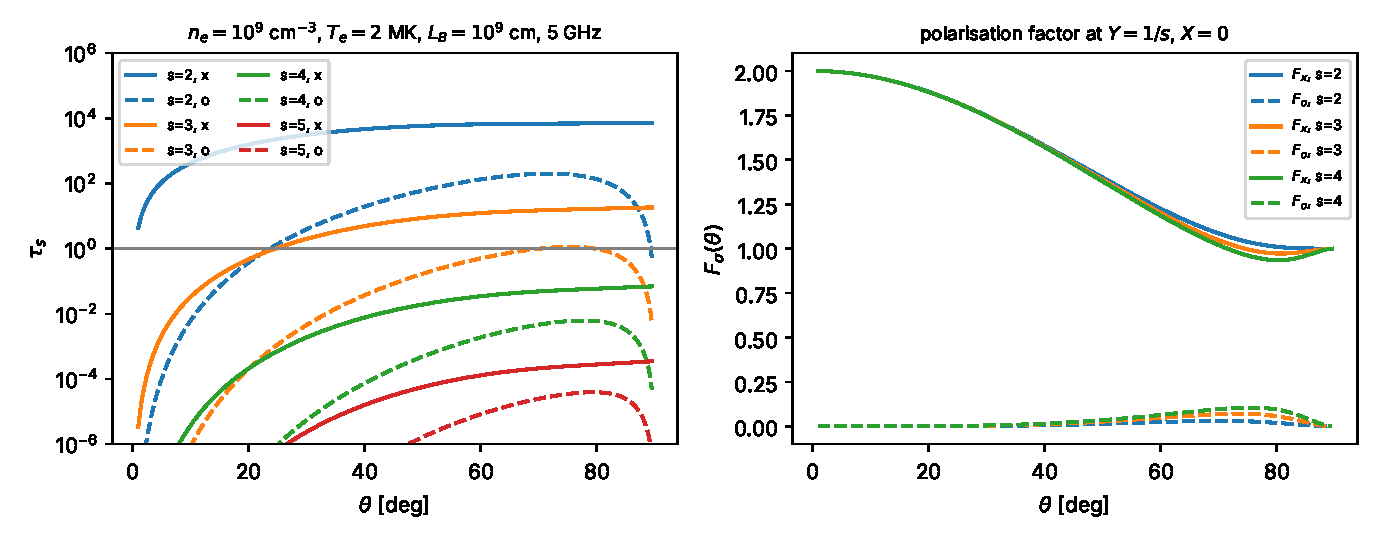
\includegraphics[width=\textwidth]{tau_theta.pdf}
\caption{Left: optical depth of the shells $s=2$--5 against the angle $\theta$ between the field and
the line of sight (solid: x-mode, dashed: o-mode; same values as in Chapter~3). Right: the
polarisation factor $F$ of the two modes. Computed with \textsf{radiosynth}.}
\label{fig:tau}
\end{figure}

\keyidea{the x-mode, which rotates with the electrons, sees opaque shells; the o-mode sees much
thinner ones.}

%----------------------------------------------------------------------
\chapterhead{5.\quad An opaque shell is a thermometer}{Kirchhoff's law}

The electrons are thermal, so each mode glows exactly as much as it absorbs. Each mode carries
half of the thermal radiation,
\begin{equation}
  S=\frac{\nu^2\kB T_e}{c^2},
\end{equation}
and an opaque shell shows, in that mode, the brightness temperature $T_b=T_e$ of the gas
\emph{at the shell}. That is why a sunspot at microwaves is as hot as the corona above it: the
telescope reads the temperature of the $s=2$ or $s=3$ shell, and as the frequency changes, the
shell --- and the height we read the temperature at --- moves.

\keyidea{where a shell is opaque, we read the coronal temperature at the height of that shell.}

%----------------------------------------------------------------------
\chapterhead{6.\quad Walking along the line of sight}{What the computer does}

At microwaves the plasma is far too thin to bend the rays, so \textsf{radiosynth} uses
\emph{straight} lines of sight, one per pixel. Along each line it:

\begin{enumerate}[label=\textbf{\arabic*.}]
\item \textbf{samples the model} at equally spaced points: density $n_e$, temperature $T_e$ and
      the field $\vect B$ (strength and angle $\theta$ to the line of sight);
\item \textbf{looks between each pair of points for a shell}: a shell lies there if $s\nuB-\nu$
      changes sign. It finds where by interpolation, and estimates the thickness scale from the
      change of field over the step,
      \begin{equation}
        L_B=\frac{B_s\,\Delta\ell}{|B_{k+1}-B_k|};
      \end{equation}
\item \textbf{computes the shell's optical depth} with Eq.~\eqref{eq:tau}, for both modes, plus the
      ordinary free--free absorption of the step (slightly different for the two modes in a
      field);
\item \textbf{adds the light} of each step, dimmed by everything in front of it,
      \begin{equation}
        I\ \leftarrow\ I+S\left(1-e^{-\Delta\tau}\right)e^{-\tau},\qquad \tau\leftarrow\tau+\Delta\tau,
      \end{equation}
      once for each polarisation, from the observer inwards.
\end{enumerate}
The shells are much thinner than a step, but that does not matter: the code does not need to see
inside a shell, only to know that the line of sight crossed it.

\keyidea{straight lines; find the shells between sample points; add their opacity and glow, one
polarisation at a time.}

%----------------------------------------------------------------------
\chapterhead{7.\quad Left or right: the field tells us its direction}{Circular polarisation}

Where the field points towards the observer, the x-mode is right-handed; where it points away,
left-handed. So \textsf{radiosynth} follows the right-handed ($R$) and the left-handed ($L$)
light separately, each using the x-mode or the o-mode opacity depending on the field direction in
each step, and gives
\begin{equation}
  I=R+L,\qquad V=R-L,\qquad \frac{V}{I}\ \text{between}\ -1\ \text{and}\ +1 .
\end{equation}
If a layer is opaque in the x-mode but transparent in the o-mode, almost all the light is in one
hand and $|V/I|\to1$; if it is opaque in both, $V\to0$. The sign of $V$ is the sign of the field.
(Where the field turns across the line of sight, the light either keeps its hand --- \emph{weak
coupling}, the default --- or keeps its mode --- \emph{strong coupling}; both can be chosen.)

\keyidea{$V=R-L$ maps the polarity of the field; its size tells which modes are opaque.}

%----------------------------------------------------------------------
\chapterhead{8.\quad The picture}{A bipolar active region at 5 and 17\,GHz}

Fig.~\ref{fig:images} shows what \textsf{radiosynth} computes for a model active region with two
spots of opposite polarity, a 2.5\,MK corona and fields up to 2500\,G.

\begin{figure}[ht]
\centering
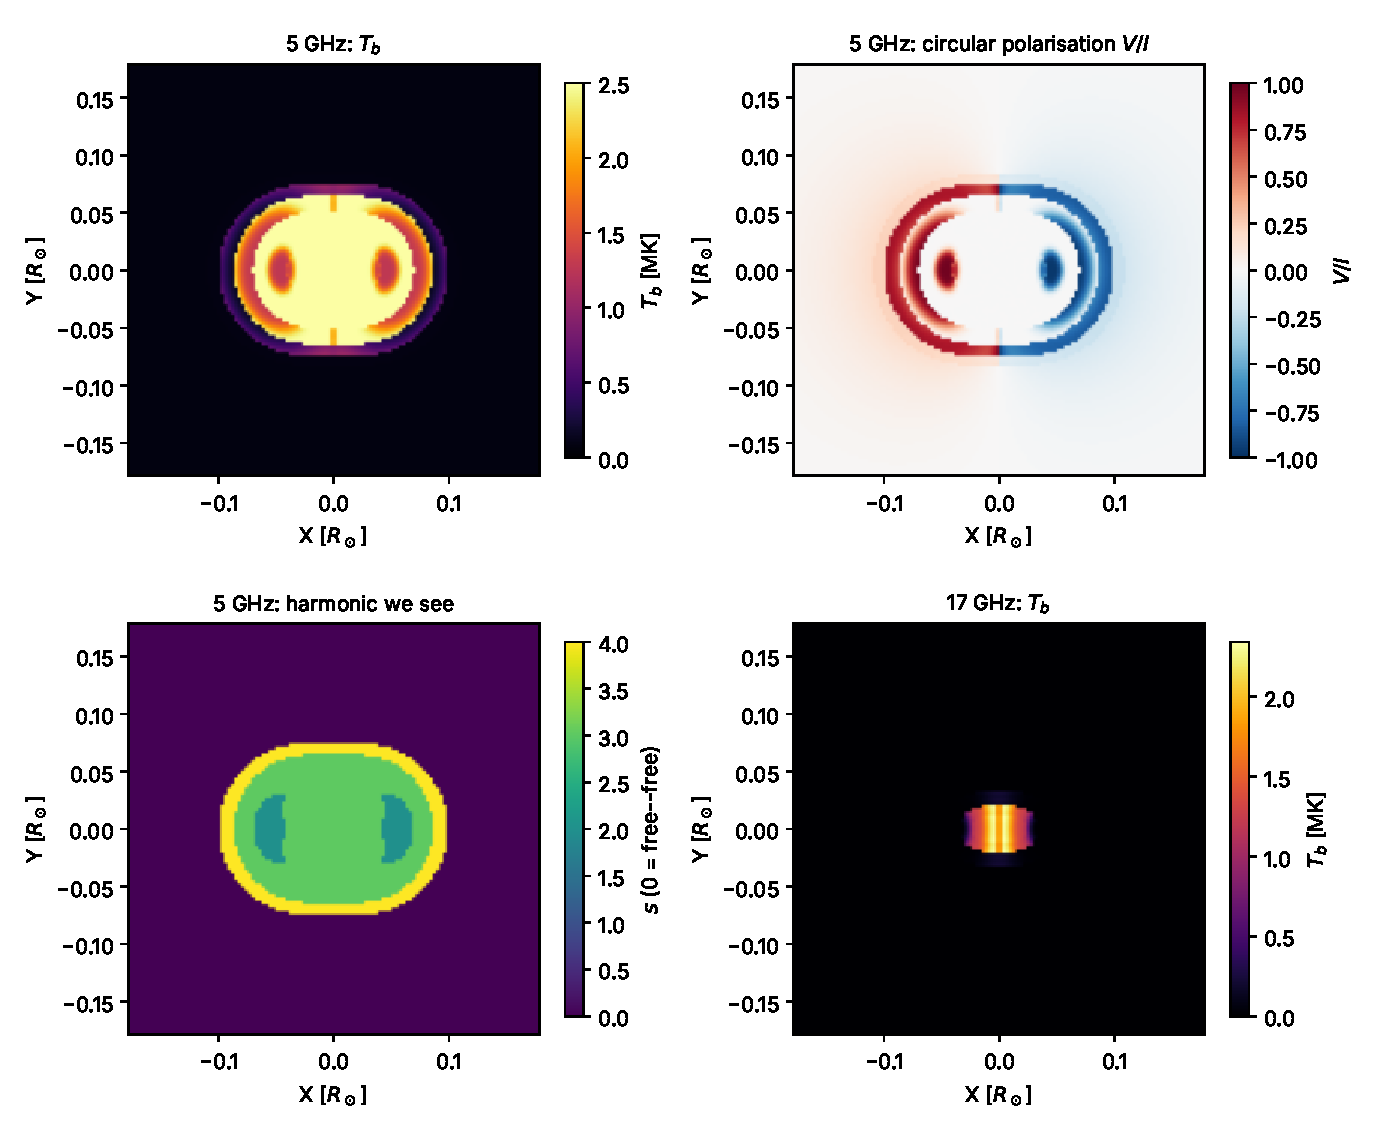
\includegraphics[width=0.82\textwidth]{gr_story_images.pdf}
\caption{Gyroresonance and free--free emission of a model bipolar active region seen from above,
computed with \code{rs.make\_gr\_image}. Top left: brightness temperature at 5\,GHz; top right: circular
polarisation $V/I$ at 5\,GHz; bottom left: the harmonic that produces most of the light at 5\,GHz (0 means
free--free); bottom right: brightness temperature at 17\,GHz.}
\label{fig:images}
\end{figure}

The story of the previous chapters can be read directly from the picture:
\begin{itemize}
\item \textbf{The source is as hot as the corona.} At 5\,GHz most of the region shows
      $T_b=2.5$\,MK $=T_e$: the line of sight crosses the opaque $s=3$ shell (green in the third
      panel). The total flux is 89\,sfu, against 18\,sfu and at most 0.45\,MK from free--free alone.
\item \textbf{The edge is the $s=4$ shell} (yellow ring), which is only partly opaque, so the
      source fades there.
\item \textbf{The spot centres are darker and fully polarised.} There the field points almost
      straight at us, $\sin\theta\to0$: the shells become thin (Chapter~3), only the x-mode is still
      opaque, at $s=2$, and the light is almost all of one hand, $|V/I|\approx1$. Each spot is
      polarised with the sign of its field --- red ($V>0$) for the one pointing to us, blue for the
      other --- and for this symmetric pair the total $V$ is zero.
\item \textbf{At 17\,GHz the source shrinks.} The shells now need $B_3\approx2000$\,G, which
      exists only low down, so only a small core between the spots, where the field is strong and
      seen across the line of sight, stays bright.
\end{itemize}

%----------------------------------------------------------------------
\chapterhead{9.\quad The whole story in six lines}{}

\begin{enumerate}[label=\textbf{\arabic*.}]
\item Electrons spiral in the field at $\nuB=2.8$\,MHz per gauss.
\item At frequency $\nu$ they absorb and emit only in thin shells where $\nu=s\nuB$.
\item The shell opacity falls by a factor of several hundred per harmonic, so only $s=2$ and 3 are opaque; shells
      seen along the field are thin.
\item The x-mode, rotating with the electrons, is far more opaque than the o-mode.
\item An opaque shell shows the temperature of the corona at its height.
\item Following right- and left-handed light along straight lines gives $I$, and $V$, whose sign
      is the sign of the field.
\end{enumerate}

In \textsf{radiosynth} all of this is one line:
\begin{small}
\begin{verbatim}
img = rs.make_gr_image(grid, "5GHz, 17GHz", x_size=0.4, y_size=0.4)
img.plot("tb"); img.plot("pol"); img.plot("harmonic")
\end{verbatim}
\end{small}
and every equation, with the code that implements it, is in the companion note \emph{Thermal
gyroresonance emission in radiosynth}.

\vspace{6pt}
{\small\textbf{Further reading.} White \& Kundu 1997, Sol.\ Phys.\ 174, 31 (gyroresonance emission
from coronal magnetic fields); Dulk 1985, ARA\&A 23, 169; Zheleznyakov 1970, \emph{Radio Emission of
the Sun and Planets}.}

\end{document}
